\documentclass[runningheads]{llncs}
\usepackage[T1]{fontenc}
\usepackage{lmodern}
\usepackage[utf8]{inputenc}
\usepackage[spanish]{babel}
\usepackage{graphicx}
\usepackage{booktabs}
\usepackage{array}
\usepackage{url}
\usepackage{float}
\usepackage{listings}
\usepackage{xcolor}
\usepackage{amsmath}
\emergencystretch=3em
\raggedbottom
\setlength{\intextsep}{8pt plus 2pt minus 2pt}

\lstset{
  language=SQL, basicstyle=\ttfamily\scriptsize, keywordstyle=\bfseries,
  commentstyle=\itshape\color{gray}, frame=single, framerule=0.3pt,
  breaklines=true, columns=fullflexible, showstringspaces=false,
  literate={á}{{\'a}}1 {é}{{\'e}}1 {í}{{\'i}}1 {ó}{{\'o}}1 {ú}{{\'u}}1
           {ñ}{{\~n}}1 {Á}{{\'A}}1 {É}{{\'E}}1 {Í}{{\'I}}1 {Ó}{{\'O}}1 {Ú}{{\'U}}1
}

\begin{document}

\title{Localización de una planta agroindustrial frente al Superniño mediante AHP resuelto con lenguaje SQL - Continuación del Módulo 1}
\titlerunning{Localización con AHP y SQL}

\author{Kemelmajer, Sara (Leg. 14419) \\
Martinez, Rocío Ana (Leg. 14912) \\
Mujica, María Pilar (Leg. 14736) \\
Salamone, Lucía (Leg. 14669) }
\authorrunning{Kemelmajer, Martinez, Mujica, Salamone}

\institute{Facultad de Ingeniería, Universidad Nacional de Cuyo, Mendoza, Argentina
\url{https://ingenieria.uncuyo.edu.ar}}

\maketitle

\begin{abstract}
En el Módulo 1 se eligió, con el proceso analítico jerárquico (AHP), el tema del proyecto final: planificación de la producción en agroindustria bajo la variabilidad climática del Superniño. En este trabajo se toma la siguiente decisión del proyecto, correspondiente al capítulo de tamaño y localización del Manual de proyectos: en qué parque industrial de Mendoza ubicar la planta. Se compararon cinco parques según cinco criterios. A diferencia del Módulo 1, todo el modelo se implementó en una base de datos SQLite: los juicios, los datos reales de los parques y los cálculos del AHP (pesos, consistencia, prioridades, ranking y sensibilidad) son tablas y consultas SQL. El parque PASIP de Palmira resultó el mejor ubicado (31,6~\%), seguido por el Área Industrial Acceso Sur (25,3~\%).
\end{abstract}

\section{Introducción}
El capítulo IV del Manual de proyectos~\cite{melnick} trata el tamaño y la localización del proyecto. Allí la localización se analiza a partir de las \emph{fuerzas locacionales}: el transporte, la disponibilidad y el costo de los insumos (mano de obra, materias primas, agua, energía) y otros factores como el clima y las facilidades de la zona. Para un proyecto agroindustrial expuesto al Superniño se agrega una fuerza más: el riesgo de que la planta quede en una zona inundable.

El Módulo 1 resolvió el AHP con una calculadora web. Aquí se propuso resolverlo con el lenguaje SQL, por tres motivos:
\begin{enumerate}
\item Los datos de las alternativas (empleo, superficie, riesgo hídrico, viñedos) ya existen en tablas generadas en el Módulo 3~\cite{modulo3}; una base de datos permite usarlos directamente en lugar de convertirlos en juicios subjetivos.
\item Las operaciones del AHP (sumar columnas, normalizar, promediar filas, ponderar) se expresan con \texttt{JOIN}, \texttt{GROUP BY} y funciones de ventana.
\item Cambiar un juicio o un dato y recalcular todo es inmediato, lo que facilita el análisis de sensibilidad.
\end{enumerate}

\section{Herramientas y método}
Se utilizó SQLite~\cite{sqlite} (versión 3.25 o posterior, por las funciones de ventana) y el programa DB Browser for SQLite~\cite{dbbrowser} para ejecutar el script y visualizar las tablas. El script \texttt{localizacion.sql} crea la base desde cero, y la base \texttt{localizacion.db} se entrega ya construida.

El AHP~\cite{saaty1980} se aplicó así:
\begin{itemize}
\item \textbf{Pesos de los criterios:} comparación por pares en la escala de Saaty (1 a 9). Se carga sólo el triángulo superior de la matriz; los recíprocos y la diagonal los genera una vista. Los pesos se obtienen normalizando cada columna y promediando cada fila (método aproximado del autovector).
\item \textbf{Consistencia:} se calcula $\lambda_{max}$, el índice $CI=(\lambda_{max}-n)/(n-1)$ y la razón $CR=CI/RI$, que debe ser menor a 0,10.
\item \textbf{Prioridades de las alternativas:} en los cuatro criterios con dato medible, el valor de cada parque se convierte linealmente a la escala 1--9 (el mejor recibe 9 y el peor 1) y luego se normaliza para que sume 1. En la logística, que no tiene un dato único, se usaron comparaciones por pares.
\item \textbf{Puntaje global:} suma de peso del criterio por prioridad local.
\end{itemize}

\section{Modelo de datos}
La base tiene nueve tablas (Fig.~\ref{fig:er}). Las tablas \texttt{departamento} y \texttt{parque} guardan los datos reales; \texttt{criterio}, \texttt{comparacion\_criterios} y \texttt{comparacion\_logistica} guardan los juicios con su justificación; \texttt{escenario} y \texttt{escenario\_peso}, los escenarios de sensibilidad; \texttt{fuente}, el origen de cada dato, e \texttt{indice\_aleatorio}, la tabla RI de Saaty.

\begin{figure}[H]
\centering
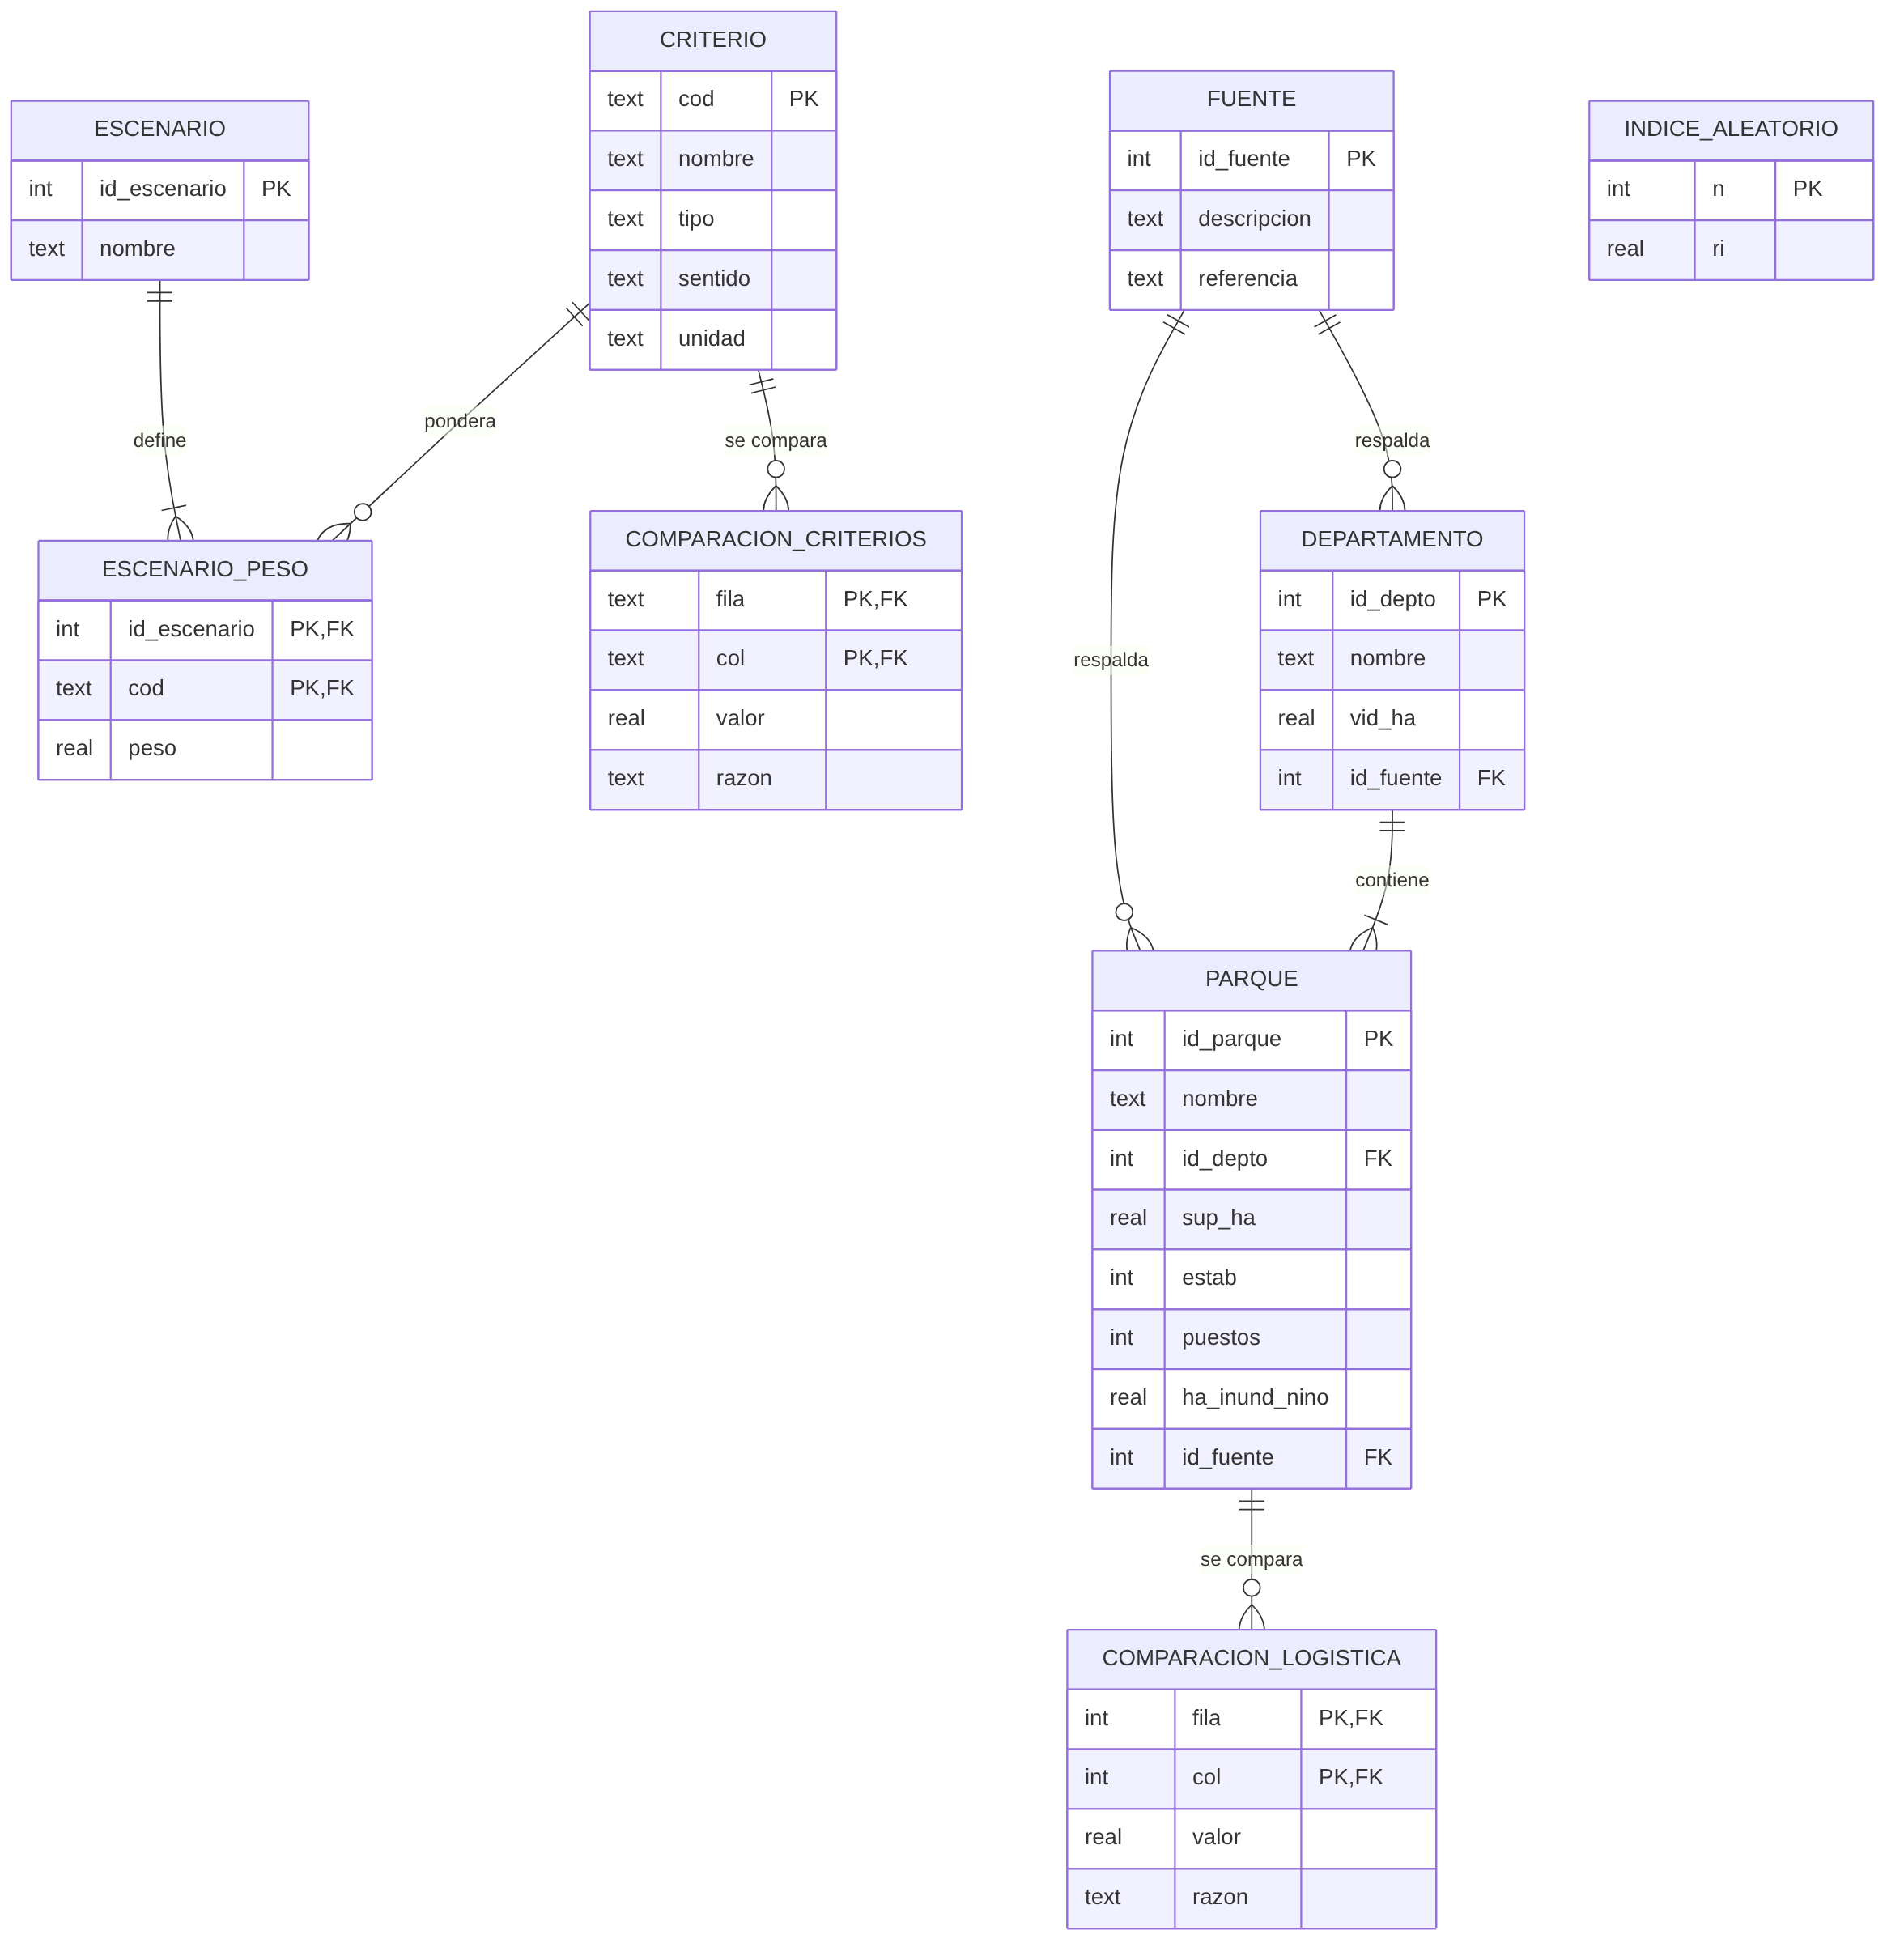
\includegraphics[width=\textwidth]{er.png}
\caption{Diagrama entidad-relación de la base \texttt{localizacion.db}.}\label{fig:er}
\end{figure}

\textbf{Normalización.} Normalizar una base es organizar sus tablas para que cada dato se guarde una sola vez y dependa sólo de la clave de su tabla. Así se evitan repeticiones y contradicciones al actualizar. El modelo cumple las tres primeras formas normales:
\begin{itemize}
\item \textbf{1FN:} cada celda tiene un único valor. Las matrices de comparación no se guardan como grillas sino como filas \emph{(fila, col, valor)}.
\item \textbf{2FN:} en las tablas con clave compuesta, como \texttt{escenario\_peso} (\texttt{id\_escenario}, \texttt{cod}), el peso depende de la clave completa. El nombre del escenario va en su propia tabla.
\item \textbf{3FN:} no hay dependencias entre columnas que no son clave. La superficie de vid es un dato del departamento, no del parque, por lo que se guarda en \texttt{departamento} y se obtiene con un \texttt{JOIN}. Así no se repite en los dos parques de Junín ni en los dos de Luján de Cuyo.
\end{itemize}

\section{Alternativas y criterios}
Se eligieron cinco parques del Módulo 3 que ofrecen contraste en riesgo, tamaño y ubicación (Cuadro~\ref{tab:datos}).

\begin{table}[H]
\centering
\small
\caption{Alternativas y datos de cada criterio. Fuentes: Módulo 3 (Tablas 2 y 6)~\cite{modulo3} e INV (2018)~\cite{inv2018}.}\label{tab:datos}
\begin{tabular}{lllrrrr}
\toprule
Parque & Dpto. & & R (ha) & M (puestos) & S (estab/ha) & P (ha vid)\\
\midrule
PASIP Palmira & San Martín & & 0,0 & 405 & 0,10 & 28\,423\\
ZI San Roque & Junín & & 264,2 & 347 & 0,13 & 11\,477\\
PI Provincial (PIP) & Luján de Cuyo & & 76,3 & 1\,303 & 0,05 & 15\,543\\
AI Acceso Sur & Luján de Cuyo & & 42,6 & 7\,180 & 1,17 & 15\,543\\
PI Los Barriales & Junín & & 0,0 & 61 & 0,11 & 11\,477\\
\bottomrule
\end{tabular}
\end{table}

Los criterios fueron:
\begin{enumerate}
\item \textbf{R - Riesgo hídrico en año Niño} (menor es mejor): hectáreas potencialmente inundables a 500~m o menos del parque, en el escenario de crecida Niño (HAND $\le$ 3~m) del Módulo 3.
\item \textbf{P - Cercanía a la materia prima} (mayor es mejor): superficie de vid del departamento, la principal agroindustria de Mendoza.
\item \textbf{L - Acceso logístico}: conexión con las rutas troncales (RN~7 y RN~40) y con el ferrocarril. Se evaluó por comparación por pares.
\item \textbf{S - Suelo disponible} (menor es mejor): establecimientos instalados por hectárea de parque, como indicador de ocupación.
\item \textbf{M - Mano de obra y ecosistema industrial} (mayor es mejor): puestos de trabajo estimados en el parque.
\end{enumerate}

\section{Pesos de los criterios}

\begin{table}[H]
\centering
\small
\caption{Comparación por pares de los criterios.}\label{tab:compcrit}
\begin{tabular}{|p{1.9cm}|p{1cm}|p{0.8cm}|p{6.7cm}|}
\hline
Comparación & Gana & Valor & Razón\\
\hline
R vs P & R & 2 & El proyecto trata sobre el Superniño: una planta inundable invalida lo demás\\
R vs L & R & 3 & La logística se compensa con transporte; una crecida no\\
R vs S & R & 4 & El suelo se consigue; el riesgo no se elige\\
R vs M & R & 5 & La mano de obra del oasis se traslada en distancias cortas\\
P vs L & P & 2 & La uva es perecedera: conviene procesarla cerca de la finca\\
P vs S & P & 3 & Sin materia prima cercana el suelo barato no sirve\\
P vs M & P & 4 & Mismo motivo\\
L vs S & L & 2 & Acceso a RN~7 y RN~40 para despachar a Chile y a Buenos Aires\\
L vs M & L & 2 & Mismo motivo\\
S vs M & Igual & 1 & Ambos son secundarios\\
\hline
\end{tabular}
\end{table}

La consulta que calcula los pesos es:
\begin{lstlisting}
CREATE VIEW v_pesos_criterios AS
  WITH suma_col AS (
    SELECT col, SUM(valor) AS s FROM v_matriz_criterios GROUP BY col)
  SELECT m.fila AS cod, AVG(m.valor / sc.s) AS peso
  FROM v_matriz_criterios m JOIN suma_col sc ON sc.col = m.col
  GROUP BY m.fila;
\end{lstlisting}

\begin{table}[H]
\centering
\small
\caption{Pesos de los criterios ($\lambda_{max}=5,035$; CR $=0,8$~\%).}\label{tab:pesos}
\begin{tabular}{lrc}
\toprule
Criterio & Peso (\%) & Posición\\
\midrule
R - Riesgo hídrico en año Niño & 42,1 & 1\\
P - Cercanía a la materia prima & 26,6 & 2\\
L - Acceso logístico & 14,9 & 3\\
S - Suelo disponible & 8,6 & 4\\
M - Mano de obra y ecosistema & 7,8 & 5\\
\bottomrule
\end{tabular}
\end{table}

La vista \texttt{v\_consistencia\_criterios} devuelve CR $=0,008$, muy por debajo de 0,10, por lo que los juicios son consistentes.

\section{Prioridades de las alternativas}
\subsection{Criterios con dato}
Para los criterios R, P, S y M, la vista \texttt{v\_escala} lleva cada valor a la escala 1--9 con la expresión
\begin{align*}
s &= 1 + 8\,\frac{x - x_{min}}{x_{max} - x_{min}} && \text{(mayor es mejor)}\\
s &= 1 + 8\,\frac{x_{max} - x}{x_{max} - x_{min}} && \text{(menor es mejor)}
\end{align*}
y la vista \texttt{v\_prioridad\_local} divide cada puntaje por la suma del criterio usando una función de ventana:
\begin{lstlisting}
SELECT id_parque, cod,
       puntaje_1a9 / SUM(puntaje_1a9) OVER (PARTITION BY cod) AS prioridad
FROM v_escala;
\end{lstlisting}

\subsection{Logística}
Al no existir un indicador único de accesibilidad, se compararon los parques por pares (Cuadro~\ref{tab:complog}). La matriz obtuvo CR $=0,1$~\%.

\begin{table}[H]
\centering
\small
\caption{Comparación por pares de los parques según el acceso logístico.}\label{tab:complog}
\begin{tabular}{|p{3.4cm}|p{1.6cm}|p{0.8cm}|p{5.1cm}|}
\hline
Comparación & Gana & Valor & Razón\\
\hline
Acceso Sur vs PIP y PASIP & Acceso Sur & 2 & Sobre la RN~40, junto al Gran Mendoza y a la RN~7\\
Acceso Sur vs San Roque y Los Barriales & Acceso Sur & 5 & Estos dos quedan lejos de las rutas troncales\\
PIP vs PASIP & Igual & 1 & PIP: RN~7 hacia Chile; PASIP: RN~7 hacia el este y nodo ferroviario de Palmira\\
PIP y PASIP vs San Roque y Los Barriales & PIP y PASIP & 3 & Mejor conexión troncal\\
San Roque vs Los Barriales & Igual & 1 & Ambos en Junín, accesos similares\\
\hline
\end{tabular}
\end{table}

\section{Resultados}

\begin{table}[H]
\centering
\small
\caption{Prioridades locales (L) y aporte al puntaje global (G, en puntos \%).}\label{tab:resultados}
\setlength{\tabcolsep}{4pt}\begin{tabular}{lrrrrrrrrrrr}
\toprule
 & & \multicolumn{2}{c}{PASIP} & \multicolumn{2}{c}{San Roque} & \multicolumn{2}{c}{PIP} & \multicolumn{2}{c}{Acc. Sur} & \multicolumn{2}{c}{L. Barriales}\\
\cmidrule(lr){3-4}\cmidrule(lr){5-6}\cmidrule(lr){7-8}\cmidrule(lr){9-10}\cmidrule(lr){11-12}
Crit. & Peso & L & G & L & G & L & G & L & G & L & G\\
\midrule
R & 0,421 & 0,269 & 11,3 & 0,030 & 1,3 & 0,200 & 8,4 & 0,231 & 9,7 & 0,269 & 11,3\\
P & 0,266 & 0,534 & 14,2 & 0,059 & 1,6 & 0,173 & 4,6 & 0,173 & 4,6 & 0,059 & 1,6\\
L & 0,149 & 0,220 & 3,3 & 0,076 & 1,1 & 0,220 & 3,3 & 0,409 & 6,1 & 0,076 & 1,1\\
S & 0,086 & 0,243 & 2,1 & 0,236 & 2,0 & 0,253 & 2,2 & 0,028 & 0,2 & 0,241 & 2,1\\
M & 0,078 & 0,092 & 0,7 & 0,087 & 0,7 & 0,159 & 1,2 & 0,596 & 4,6 & 0,066 & 0,5\\
\midrule
Total & 1,000 & & 31,6 & & 6,7 & & 19,7 & & 25,3 & & 16,6\\
\bottomrule
\end{tabular}
\end{table}

La vista \texttt{v\_ranking} ordena los parques con \texttt{RANK() OVER}. El ranking final es:
\begin{enumerate}
\item PASIP Palmira (San Martín): 31,6~\%.
\item AI Acceso Sur (Luján de Cuyo): 25,3~\%.
\item PI Provincial (Luján de Cuyo): 19,7~\%.
\item PI Los Barriales (Junín): 16,6~\%.
\item ZI San Roque (Junín): 6,7~\%.
\end{enumerate}

\begin{figure}[H]
\centering
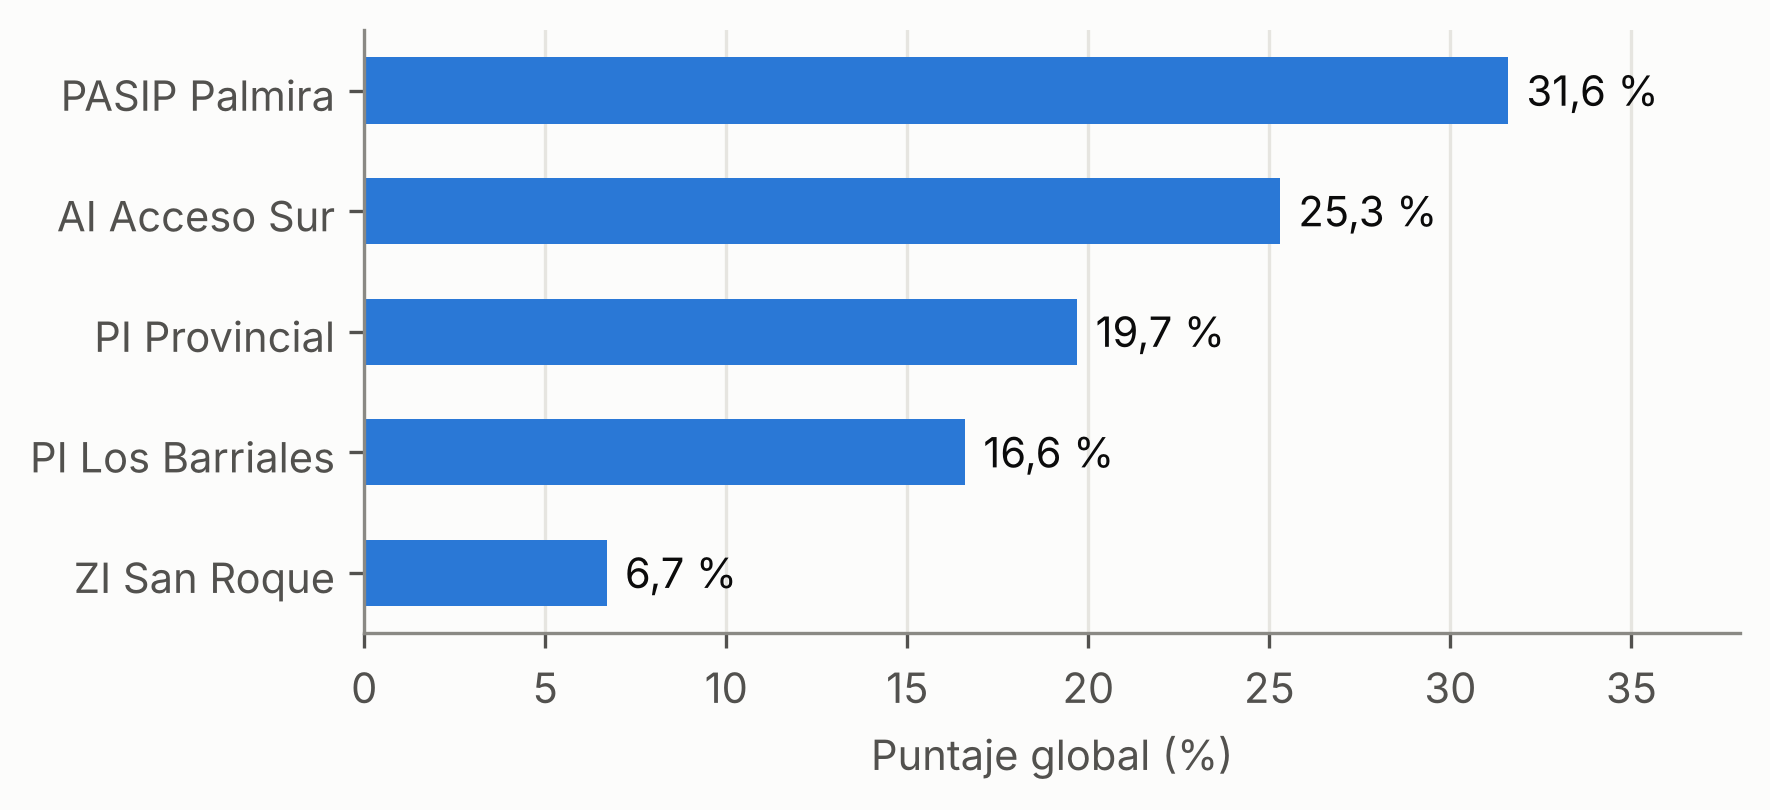
\includegraphics[width=0.8\textwidth]{ranking.png}
\caption{Ranking final (puntaje global).}\label{fig:ranking}
\end{figure}

\begin{figure}[H]
\centering
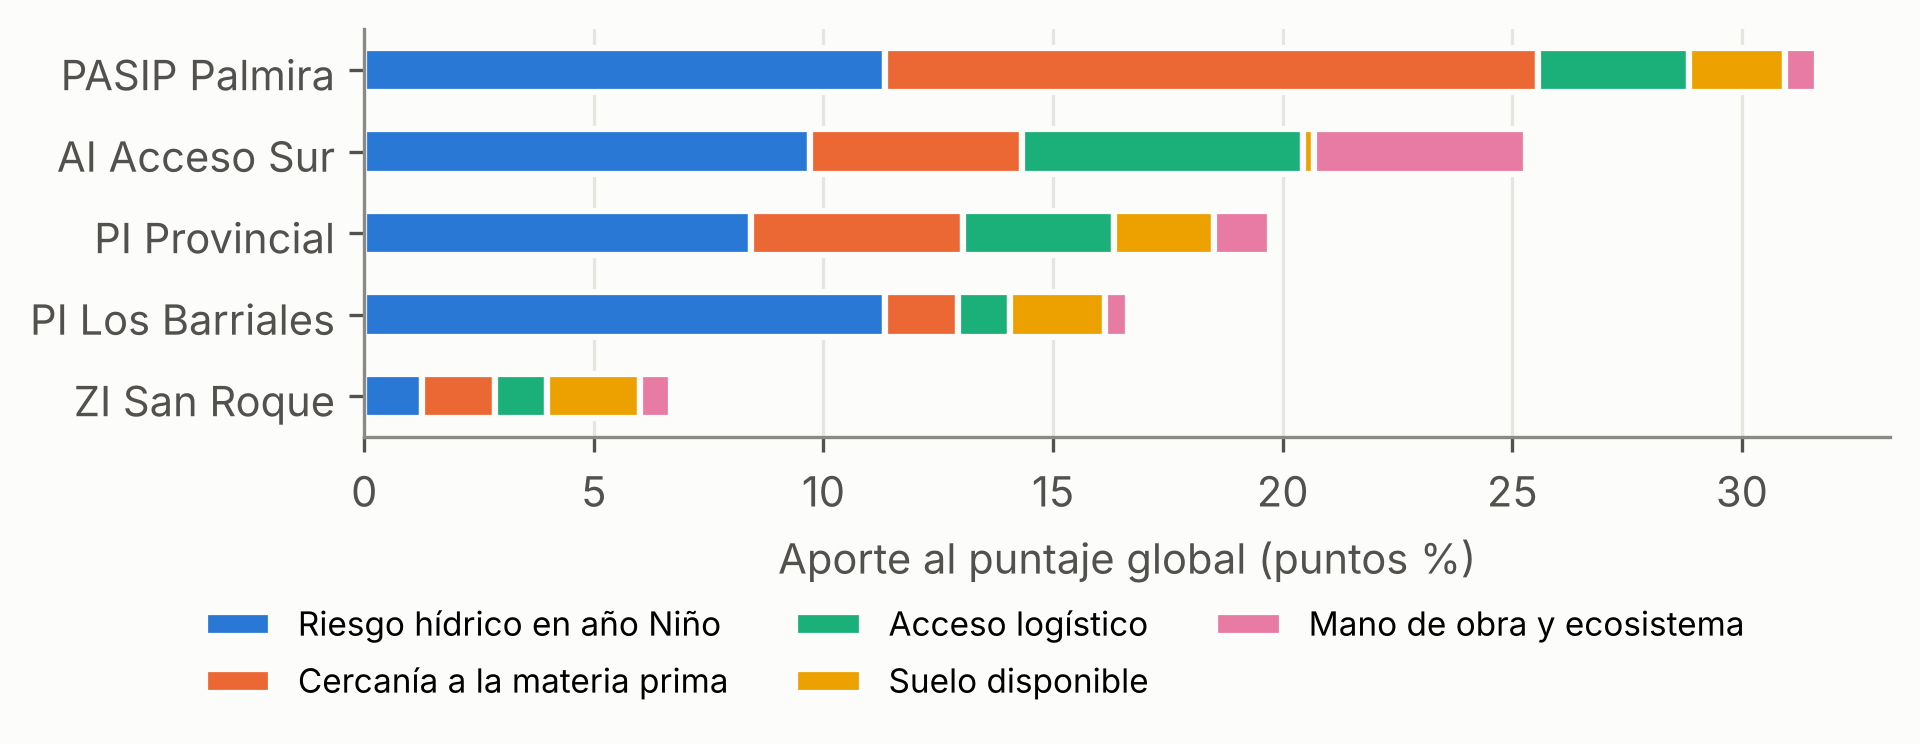
\includegraphics[width=0.9\textwidth]{aporte.png}
\caption{Aporte de cada criterio al puntaje global de cada parque.}\label{fig:aporte}
\end{figure}

PASIP gana por la combinación de los dos criterios más pesados: no tiene superficie inundable cercana y está en San Martín, el departamento con más viñedos de la provincia, que aporta 14,2 de sus 31,6 puntos. Acceso Sur es el mejor en logística y en mano de obra, pero tiene superficie inundable cercana, casi no tiene suelo libre y su departamento tiene la mitad de viñedos que San Martín. Los Barriales empata con PASIP en riesgo, pero pierde en todos los demás criterios. San Roque queda último por su alta exposición hídrica, que coincide con la clasificación ``Alta'' del Módulo 3.

\section{Análisis de sensibilidad}
Los pesos surgen de juicios subjetivos, por lo que se evaluó cómo cambia el resultado si cambian. Los pesos de cada escenario se cargan en la tabla \texttt{escenario\_peso}, y la vista \texttt{v\_escenarios} calcula todos los puntajes en una sola consulta.

\begin{table}[H]
\centering
\small
\caption{Escenarios de ponderación (pesos y puntajes en \%).}\label{tab:escenarios}
\setlength{\tabcolsep}{3.5pt}\begin{tabular}{lrrrrrrrrrrl}
\toprule
 & \multicolumn{5}{c}{Peso del criterio (\%)} & \multicolumn{5}{c}{Puntaje (\%)} & \\
\cmidrule(lr){2-6}\cmidrule(lr){7-11}
Escenario & R & P & L & S & M & PAS & AS & PIP & LB & SR & Ganador\\
\midrule
Base (AHP) & 42,1 & 26,6 & 14,9 & 8,6 & 7,8 & \textbf{31,6} & 25,3 & 19,7 & 16,6 & 6,7 & PASIP\\
Pesos iguales & 20 & 20 & 20 & 20 & 20 & 27,2 & \textbf{28,7} & 20,1 & 14,2 & 9,8 & Acc. Sur\\
Riesgo bajo & 20 & 30 & 25 & 15 & 10 & \textbf{31,5} & 26,4 & 20,1 & 13,3 & 8,7 & PASIP\\
Logística alta & 25 & 20 & 40 & 7,5 & 7,5 & 28,7 & \textbf{30,3} & 20,3 & 13,3 & 7,4 & Acc. Sur\\
Mano de obra alta & 25 & 20 & 15 & 10 & 30 & 25,9 & \textbf{33,5} & 19,1 & 13,5 & 8,1 & Acc. Sur\\
Sin riesgo & 0 & 40 & 30 & 15 & 15 & \textbf{33,0} & 28,6 & 19,7 & 9,3 & 9,5 & PASIP\\
\bottomrule
\end{tabular}
\end{table}

\begin{figure}[H]
\centering
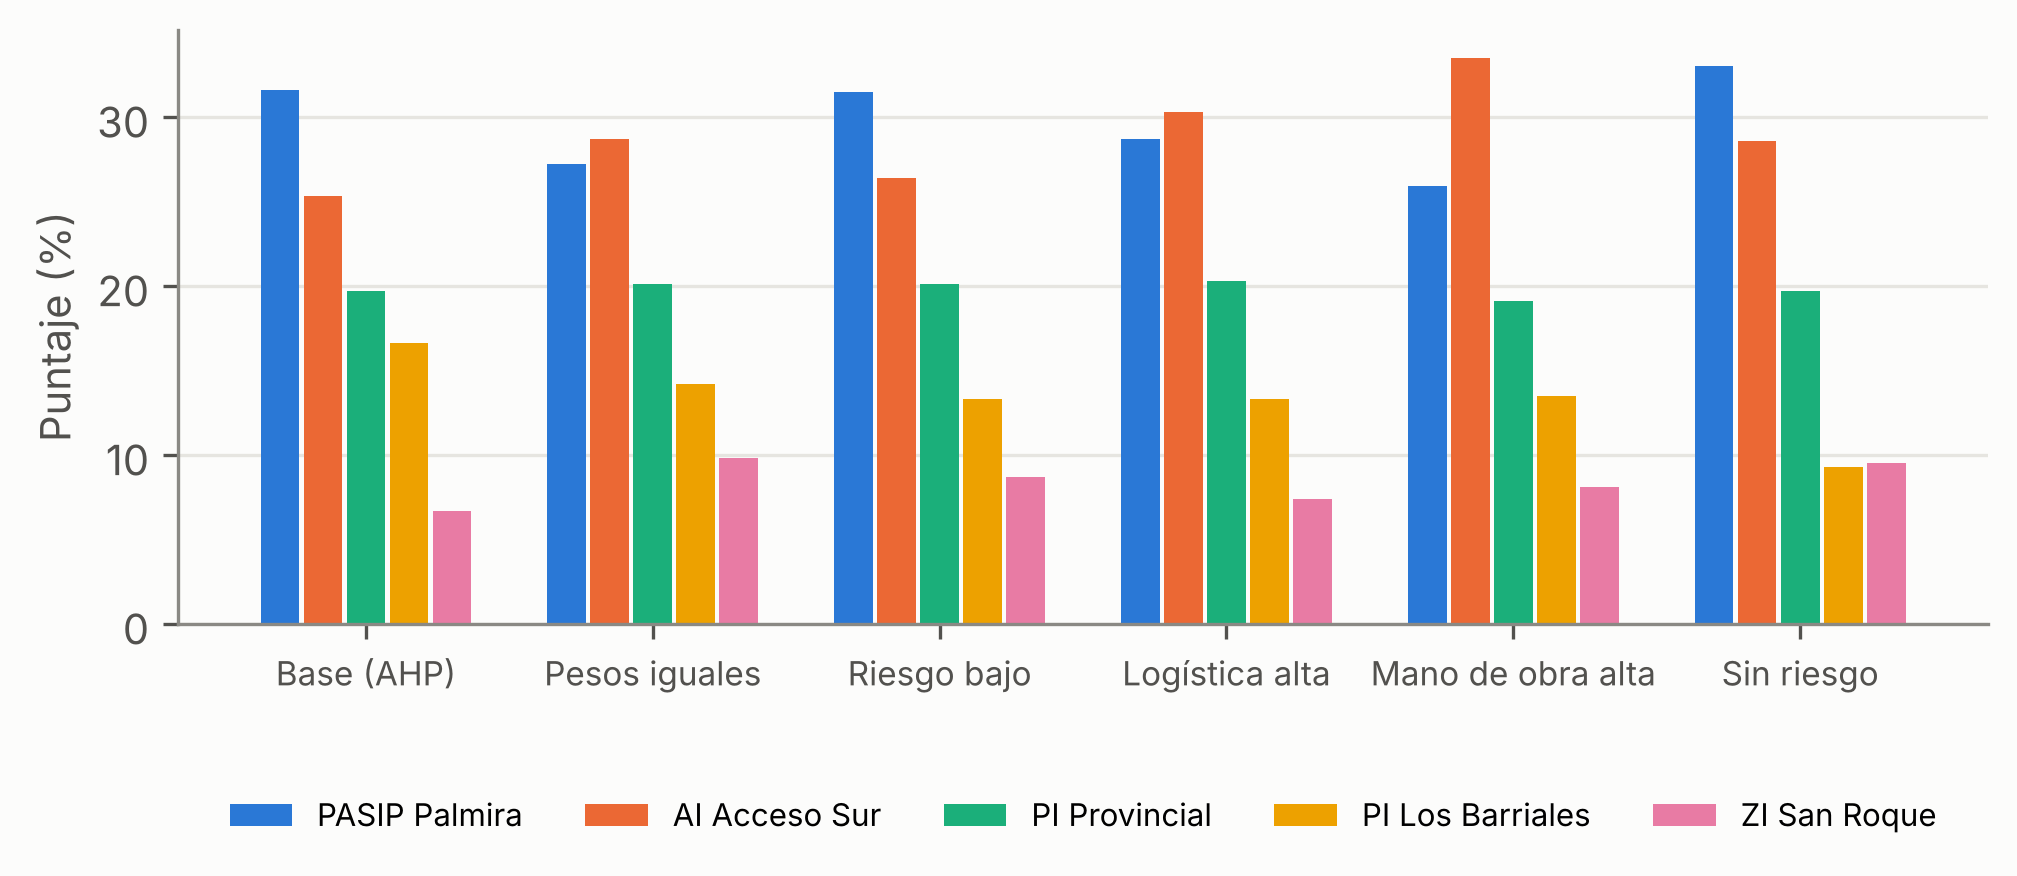
\includegraphics[width=0.95\textwidth]{escenarios.png}
\caption{Puntaje por parque en cada escenario de ponderación.}\label{fig:escenarios}
\end{figure}

Además se calculó el \emph{peso crítico} de cada criterio: el peso que debería alcanzar para que otro parque supere a PASIP, reajustando los demás pesos en forma proporcional. La vista \texttt{v\_peso\_critico} lo resuelve con un CTE recursivo que genera una grilla de pesos de 0 a 1 en pasos de 0,001:
\begin{lstlisting}
WITH RECURSIVE grilla(t) AS (
  SELECT 0.0 UNION ALL SELECT t + 0.001 FROM grilla WHERE t < 0.9995 ), ...
\end{lstlisting}

\begin{table}[H]
\centering
\small
\caption{Peso crítico de cada criterio.}\label{tab:critico}
\begin{tabular}{lrrl}
\toprule
Criterio & Peso base (\%) & Peso crítico (\%) & Nuevo ganador\\
\midrule
R - Riesgo hídrico & 42,1 & No cambia & -\\
P - Materia prima & 26,6 & 10,9 (si baja) & AI Acceso Sur\\
L - Logística & 14,9 & 36,4 (si sube) & AI Acceso Sur\\
S - Suelo disponible & 8,6 & 92,9 (si sube) & PI Provincial\\
M - Mano de obra & 7,8 & 18,1 (si sube) & AI Acceso Sur\\
\bottomrule
\end{tabular}
\end{table}

PASIP gana en el escenario base y en otros dos escenarios; Acceso Sur gana en los tres restantes. La decisión es, por lo tanto, menos robusta que la del Módulo 1 y se reduce a dos candidatos: PASIP y Acceso Sur, que suman los primeros puestos en todos los escenarios. Lo que define la elección es el peso de la materia prima frente a la logística y la mano de obra. PASIP deja de ganar si la cercanía a los viñedos pesa menos de 10,9~\%, si la logística supera 36,4~\% o si la mano de obra supera 18,1~\%. El peso del riesgo hídrico, en cambio, no altera al ganador en ningún valor, porque PASIP es el mejor (o empata) en ese criterio.

\section{Conclusión}
El AHP resuelto íntegramente con SQL indica que la planta agroindustrial del proyecto debería ubicarse en el \textbf{Parque de Actividades de Servicios e Industrias de Palmira (PASIP)}, en San Martín, con un puntaje de 31,6~\%. La elección es coherente con el Módulo 3, que recomendaba orientar plantas nuevas hacia parques de baja exposición hídrica, y con el tema del Módulo 1: una agroindustria cuyo riesgo principal es el Superniño se ubica donde no hay riesgo de crecida y donde está la materia prima.

El análisis de sensibilidad muestra que \textbf{AI Acceso Sur} es una alternativa sólida si el proyecto priorizara la logística urbana y la mano de obra. Esa comparación entre los dos finalistas debería profundizarse en el estudio de costos (capítulos V y VI del Manual), por ejemplo con el costo de flete de la uva hasta cada parque.

Respecto de la herramienta, SQL permitió guardar juicios, datos y fuentes en un mismo lugar, documentar cada juicio con su razón y recalcular todo el modelo, incluida la sensibilidad, sin repetir cálculos a mano.

\textbf{Limitaciones.} Los datos de los parques son estimaciones del Módulo 3 (CEP XXI 2022 y un índice HAND con umbrales didácticos). La superficie de vid es de 2018 y es un indicador del departamento, no de la distancia real a las fincas. La escala lineal 1--9 es una elección metodológica: comprime diferencias grandes (por ejemplo, 0 y 42,6~ha inundables quedan cerca), y otra transformación podría cambiar las prioridades. Los juicios de logística deberían validarse con un relevamiento de rutas y distancias.

\begin{thebibliography}{8}
\bibitem{saaty1980} Saaty, T.L.: The Analytic Hierarchy Process. McGraw-Hill, New York (1980)
\bibitem{melnick} Naciones Unidas, CEPAL/AAT (Melnick, J.): Manual de proyectos de desarrollo económico. Naciones Unidas, México (1958). Cap. IV: Tamaño y localización de los proyectos
\bibitem{modulo3} Kemelmajer, S., Martinez, R.A., Mujica, M.P., Salamone, L.: Módulo 3 - Geomática y Sistemas de Información Geográfica. Técnicas y Herramientas Modernas II, FING UNCuyo (2026)
\bibitem{inv2018} Instituto Nacional de Vitivinicultura: Evolución de la superficie de vid por oasis, Mendoza (2018), \url{https://www.argentina.gob.ar/sites/default/files/evolucion_de_superficie_x_oasis_mza_0.pdf}
\bibitem{sqlite} SQLite, \url{https://www.sqlite.org}
\bibitem{dbbrowser} DB Browser for SQLite, \url{https://sqlitebrowser.org}
\end{thebibliography}

\end{document}
